\begin{table}
\begin{center}
\begin{tabular}[H]{|l|}
\hline
\multicolumn{1}{|c|}{\textsc{T2a}}\\
\hline
\begin{tabular}{c|l}
\begin{minipage}{85mm}
\vspace{2mm}
\begin{center}
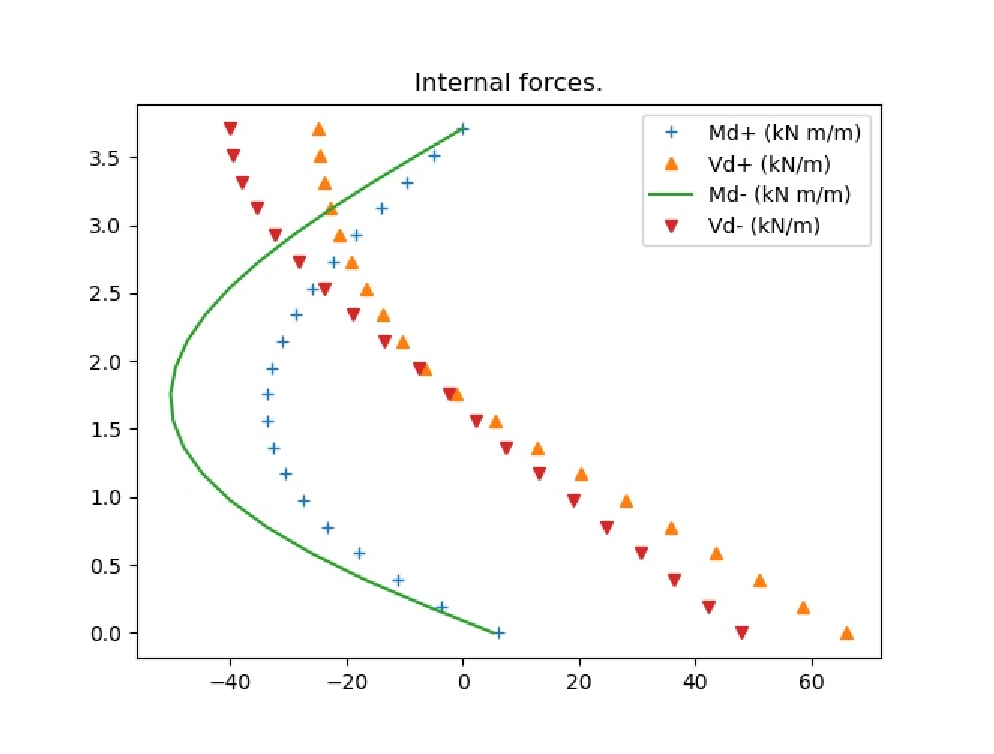
\includegraphics[width=80mm]{T2a}
\end{center}
\vspace{1pt}
\end{minipage} & 
\begin{tabular}{l}
\textsc{Géométrie mur}\\
Épaisseur couronnement: \\
$b_{couronn}= 0.25\ m$\\
Hauteur voile: \\
$h_{voile}= 3.53\ m$\\
Épaisseur encastrement: \\
$b_{encast.}= 0.25\ m$\\
Épaisseur semelle: \\
$b_{semelle.}= 0.36\ m$\\
\end{tabular} \\
\end{tabular} \\
\hline
\begin{tabular}{llll}
\multicolumn{3}{c}{\textsc{Matériels}}\\
  Béton: C3500 &   Acier: A615G60 &   ConcreteCover: 55 mm\\
\end{tabular} \\
\hline
\end{tabular}
\caption{Matériels et dimensions mur T2a} \label{tb_def_T2a}
\end{center}
\end{table}
\begin{center}
\begin{tabular}[H]{|l|c|c|c|}
\hline
\multicolumn{4}{|c|}{\textsc{Verification stabilité mur: T2a}}\\
\hline
Vérification:  & $F_{disp}$ & $F_{req}$ & Combinaison\\
\hline
Renversement:  & -270.72 & 1.00 & SR102B\\
Glissement:  & 1.51 & 1.00 & SR102A\\
Poinçonnement:  & 0.51 & 1.00 & SR102A\\
Adm. pressure:  & 0.89 & 1.00 & SR102B\\
\hline
\multicolumn{4}{|l|}{$F_{disp}$: sécurité disponible.}\\
\multicolumn{4}{|l|}{$F_{req}$: sécurité requise.}\\
\hline
\end{tabular}
\end{center}
\begin{center}
\begin{tabular}[H]{|l|c|c|c|}
\hline
\multicolumn{3}{|c|}{\textsc{Verification rotation mur: T2a}}\\
\hline
$\beta_{disp} (\permil)$ & $\beta_{req}(\permil)$ & Combinaison\\
\hline
-0.63 & 2.00 & ELS00\\
\hline
\multicolumn{3}{|l|}{$\beta_{disp}$: rotation maximale calculée du mur.}\\
\multicolumn{3}{|l|}{$\beta_{req}$: rotation maximale autorisée du mur.}\\
\hline
\end{tabular}
\end{center}
\bottomcaption{Calcul armatures mur T2a} \label{tb_T2a}
\tablefirsthead{\hline
\multicolumn{1}{|c|}{\textsc{Armatures mur T2a}}\\\hline
}
\tablehead{\hline
\multicolumn{1}{|c|}{\textsc{T2a (suite)}}\\\hline
}
\tabletail{\hline \multicolumn{1}{|r|}{../..}\\\hline}
\tablelasttail{\hline}
\begin{center}
\begin{supertabular}[H]{|l|}
\hline
\textbf{Armature 1 (armature extérieure en attente) :} \\
  Dimensions coupe; b= 1.00m, h= 0.25m\\
  diam: 16 mm, spacing: 300 mm  l. ancrage L=0.37 m (23 diamètres).\\
  diam: 19 mm, spacing: 300 mm  l. ancrage L=0.65 m (34 diamètres).\\
  area: As=  16.13 cm2/m areaMin:   4.56 cm2/m  F(As)= 3.54 OK!\\
  Verif. en flexion: Md=   2.65 kN m, MR=  99.62kN m  F(M)= 37.54 OK!\\
  Vérif. eff. tranchant: Vd=  56.40kN,  VR= 186.49kN  F(V)= 3.31 OK!\\
  Verif. contraintes: M=   2.65 kN m, $\sigma_s$=   7.19 MPa\\
    $\sigma_{lim}$= 230.00 MPa  F($\sigma_s$)= 31.97 OK!\\
\textbf{Armature 3 (armature supérieure semelle):}\\
  Dimensions coupe; b= 1.00m, h= 0.36m\\
  diam: 16 mm, spacing: 300 mm  l. ancrage L=0.37 m (23 diamètres).\\
  diam: 19 mm, spacing: 300 mm  l. ancrage L=0.65 m (34 diamètres).\\
  area: As=  16.13 cm2/m areaMin:   6.38 cm2/m  F(As)= 2.53 OK!\\
  Verif. en flexion: Md=   1.62 kN m, MR= 152.86kN m  F(M)= 94.60 OK!\\
  Vérif. eff. tranchant: Vd=   2.78kN,  VR= 261.09kN  F(V)= 93.86 OK!\\
  Verif. contraintes: M=   1.62 kN m, $\sigma_s$=   3.13 MPa\\
    $\sigma_{lim}$= 230.00 MPa  F($\sigma_s$)= 73.50 OK!\\
\textbf{Armature 4 (armature intérieure en attente):}\\
  diam: 10 mm, spacing: 150 mm  l. ancrage L=0.30 m (32 diamètres).\\
  area: As=   4.73 cm2/m areaMin:   1.72 cm2/m  F(As)= 2.75 OK!\\
\textbf{Armature 5 (armature intérieure en voile):}\\
  Dimensions coupe; b= 1.00m, h= 0.25m\\
  diam: 16 mm, spacing: 150 mm  l. ancrage L=0.37 m (23 diamètres).\\
  area: As=  13.33 cm2/m areaMin:   4.56 cm2/m  F(As)= 2.93 OK!\\
  Verif. en flexion: Md=  49.41 kN m, MR=  82.72kN m  F(M)= 1.67 OK!\\
  Vérif. eff. tranchant: Vd=   6.54kN,  VR= 186.49kN  F(V)= 28.53 OK!\\
  Verif. contraintes: M=  49.41 kN m, $\sigma_s$= 162.12 MPa\\
    $\sigma_{lim}$= 230.00 MPa  F($\sigma_s$)= 1.42 OK!\\
\textbf{Armature 6 (armature couronnement):}\\
  Dimensions coupe; b= 1.00m, h= 0.25m\\
  diam: 13 mm, spacing: 150 mm  l. ancrage L=0.30 m (24 diamètres).\\
  area: As=   8.60 cm2/m areaMin:   4.56 cm2/m  F(As)= 1.89 OK!\\
\textbf{Armature 7 (armature trsv. inférieure semelle):}\\
  diam: 10 mm, spacing: 150 mm  l. ancrage L=0.30 m (32 diamètres).\\
  area: As=   4.73 cm2/m areaMin:   3.23 cm2/m  F(As)= 1.47 OK!\\
\textbf{Armature 8 (armature long. inférieure semelle):}\\
  diam: 16 mm, spacing: 300 mm  l. ancrage L=0.37 m (23 diamètres).\\
  diam: 19 mm, spacing: 300 mm  l. ancrage L=0.65 m (34 diamètres).\\
  area: As=  16.13 cm2/m areaMin:   6.38 cm2/m  F(As)= 2.53 OK!\\
\textbf{Armature 9 (armature long. supérieure semelle):}\\
  diam: 16 mm, spacing: 300 mm  l. ancrage L=0.37 m (23 diamètres).\\
  diam: 19 mm, spacing: 300 mm  l. ancrage L=0.65 m (34 diamètres).\\
  area: As=  16.13 cm2/m areaMin:   6.38 cm2/m  F(As)= 2.53 OK!\\
\textbf{Armature 10 (armature de peau semelle):}\\
  --\\
\textbf{Armature 11 (armature long. extérieure voile):}\\
  diam: 13 mm, spacing: 150 mm  l. ancrage L=0.30 m (24 diamètres).\\
  area: As=   8.60 cm2/m areaMin:   4.56 cm2/m  F(As)= 1.89 OK!\\
\textbf{Armature 12 (armature long. intérieure voile):}\\
  diam: 13 mm, spacing: 150 mm  l. ancrage L=0.30 m (24 diamètres).\\
  area: As=   8.60 cm2/m areaMin:   4.56 cm2/m  F(As)= 1.89 OK!\\
\textbf{Armature 13 (armature long. couronnement):}\\
  --\\
\hline
\end{supertabular}
\end{center}
